\section{Techniques}
One of the main ideas during development was the decoupling of major steps in Semap’s processing pipeline. So the project is split into three smaller part: The user interface, the processing pipeline and REST interfaces. 
The frontend website is primarily responsible for the rendering of visual elements. The computation of clusters takes place on a separate backend server, which is contacted by the website using a REST-interface on the same backend server. The following sections will be based on this trisection and elaborate in more detail on each of the components.

\subsection{User Interface}
The primary access to the Semaps application happens in form of a website, where users will get visual information about a city. As a starting point, the city of Mannheim is set. The whole website is a responsive, single page web application with following user interface elements: 
\begin{itemize}
\item a search bar, where the user can search for specific places, cities, countries, and addresses
\item Three buttons with additional information like a legend of colors, information about the project and a link to the open source repository which contains the code of the frontend
\item A map in the background with colored clusters and relevant data markers in the city
\end{itemize}

In terms of technology, Semaps is entirely developed with the help of the \textit{React}\footnote{ \url{https://reactjs.org}}. React is a \textit{JavaScript}-based frontend framework which follows component-based design philosophy. This means that the interface is broken down to small, atomic subsections, also described as components, which can be reused in the entire application.

The base functionality of modern web applications can be enhanced through so-called package managers. Because React is based on the server architecture of \textit{NodeJS}\footnote{ \url{https://www.nodejs.org}} the used package manager here is \textit{NPM}\footnote{ \url{https://npmjs.org}}, which is short for Node Package Manager. With the help of such package managers, developers can use external functionalities bundled in packages, provided by other developers. In the case of Semaps, different packages were adapted. For example the package \textit{axios}\footnote{ \url{https://github.com/axios/axios}}, which provides an easier way of handling asynchronous HTTP requests. The two main packages used were \textit{leaflet}\footnote{ \url{https://leafletjs.com}} and \textit{react-leaflet}\footnote{ \url{https://react-leaflet.js.org}}. Those packages provide functionalities to implement different map features of \textit{Open Street Maps}\footnote{ \url{http://openstreetmap.org}}. At the same time, this builds the center of the Semaps User interface.

To depict the computed clusters in the backend the defined standard format of \textit{geoJSON} files was used. A geoJSON file is a special kind of JSON files which includes a set of features. In the case of Semaps, those features were interesting data points and places, visualized by markers and the computed clusters in forms of colored rectangles. With the help of the geoJSON format, there is no major business logic necessary on the frontend. The geoJSON data is simply laid over the map and the different clusters are colored respectively.

In the end, the application is deployed with the help of \textit{Heroku}\footnote{\url{https://heroku.com/}}, a popular and easy to use Platform-as-a-Service provider.

\subsection{REST Interface}
When a request is sent to the REST interface, the server reads given parameters and schedules the crawling and clustering of the data as well as the assembly of a response in the GeoJSON format. So the interface does not execute any functional computations; it rather passes on the request to different execution modules using Java dependency injection. The REST interface itself relies on the \textit{Spring Boot} framework and is hosted at the Platform-as-a-Service provider \textit{Heroku}. Spring Boot is a framework built on top of the spring framework, which facilitates the development of web applications and requires only very little configuration overhead. So it follows the architectural notion of microservices. 


\subsection{Processing Pipeline}
A core object structure underlies the processing pipeline, which is utilized whenever the backend server is contacted by the UI website. I.e. After crawling the data from respective servers, the results are saved in internal object representations and read when the processing takes place. The core object structure is tuned towards the task of semantically clustering regions and thus facilitates the use of multiple clustering implementations with diverse libraries. The UML class diagram in figure \ref{fig:cos} summarizes the object structure:
 
\begin{figure}
  \centering
    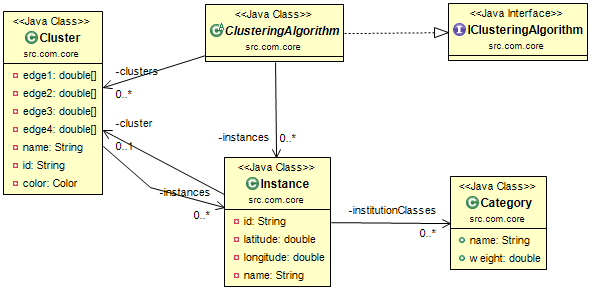
\includegraphics[scale=0.7]{./content/cos.png}
  \caption{UML class diagram of the core object structure}\label{fig:cos}
\end{figure}


The figure shows the centrality of the Instance class. All other attributes interact with it, as they rely on the information held in instance objects. Practically speaking, an instance represents a real-world institution like a specific bar or school. Each object of the instance class can have a number of Categories assigned to it. Categories make up the semantic context of an institution. They have a name like “museum” or “bar” and a weight. The semap project assumes, that the deeper a category is in its ontology, the more informative it is. That is why a detailed category like “Irish pub” is meant to get a higher weight than higher-level categories like “thing”. The clustering algorithm can then prefer to place instances based on the deep-level knowledge into clusters, resulting in more specific clusters.
Before clustering takes place, no instance is assigned to a cluster, as no cluster exists. Ideally after clustering each instance is assigned to exactly one cluster. When running a clustering algorithm (here represented by an abstract class), it will create new objects of type Cluster using a list of instances and assign those instances to a cluster. The different implementations of clustering algorithms are not depicted in the figure for abstraction purposes. But in the end, the actual implementations are of type ClusteringAlgorithm, so they just inherit from the abstract class ClusteringAlgorithm and the interface IClusteringAlgorithm. In the project, a simple square clustering algorithm and a DBScan were implemented.


\paragraph{Simple Square Clustering }
The simple square clustering algorithm a rather straight-forward implementation of clustering algorithms. It considers each element from the list of instances and creates clusters based on their position. So for each instance, the simple square clustering implementation will check if there is already a cluster, in which the current instance is located and will assign it to this cluster or create a new cluster correspondingly. After having done so for the entire list of instances, each clusters gets a category. The computation is based on a scoring function, which determines the times, a category appears in a cluster and weights each appearance by the category’s weight-property. The category with the highest weight is then allocated to a cluster. Algorithm \ref{alg:ssca} formalizes the procedures again. In sum, the simple square clustering algorithm does not take into account the semantic context (i.e. the categories) of instances and only uses positional information initially. That is why the results are not guaranteed to be semantically meaningful. However, the algorithm runs very fast, as it is linked to very little computational overhead.


\begin{algorithm}
\caption{Sketch of the simple quare clustering algorithm}\label{alg:ssca}
\begin{algorithmic} 
\STATE $I \gets \text{set~of~all~instances}$
\STATE $C \gets \emptyset$
\FORALL{$i \in I$}
\FORALL{$c \in C$}
 \IF{$i~located~in~c$}
  \STATE $c.add(i)$
  \ELSE 
  \STATE $x \gets createCluster(i.latitude, i.longitude)$
  \STATE $C \gets C \cap x$
\ENDIF
\ENDFOR
\ENDFOR
\STATE ${CAT} \gets \emptyset$
\FORALL{$i \in C.getInstances()$}
\FORALL{$category \in i.getCategories()$}
\STATE ${CAT}_{category} \gets {CAT}_{category}.getScore() + category.getScore()$
\STATE ${CAT} \gets {CAT} \cap {CAT}_{category}$
\ENDFOR
\ENDFOR
\RETURN $max({CAT}.getAllScores())$
\end{algorithmic}
\end{algorithm}

\paragraph{DBScan}
DBScan is a the sophisticated clustering algorithm in the semap project and relies on the Weka library implementation. The DBScan tries to build clusters based on two pieces of information: The position of instances and their categories. The position is determined by the longitude and latitude coordinates and is normalized on a scale from zero to one; alternatively it can be z-normalized by a parameter setting in the Java coding. Categories are one-hot-encoded, so that each instance gets a vectors consisting of values in the range from one to zero. The vector represents the set of all categories. Each category is represented by a positional value in the vector. All the categories an instance does not belong to, take the value 0 in the vector. The categories, an instance belongs to, take a normalized value greater than zero. The value is determined by the formula: 
\begin{equation}
n := number~of~categories~of~an~instance
\end{equation}
\begin{equation}
w_i := weight~of~the~i\-th~category~of~an~instance
\end{equation}
\begin{equation}
w_c := weight~of~current~category
\end{equation}
\begin{equation}\label{eq:normalization}
val = \frac{w_c}{\sum_{i=0}^{n}w_i}
\end{equation}


Weight of current category/sum of categories of an instance(weight)
So the value depends on the number of instance’s categories and the weight of the respective categories. This method ensures, that the weighted vector values have the same impact on the clustering as the positional information latitude and longitude. Before the DBScan algorithm can start working in Weka, a preprocessing pipeline transform the internal object representation as described in figure \ref{fig:cos} into the object representation needed by the Weka library. It therefore writes an artificial .arff-file to disk and reads it again with tools from the weka library. Afterwards, the DBScan is executed and the results again returned into the core object representation of semap. The entire procedure of the DBScan in the semap project is summarized in algorithm \ref{alg:dbscan} as follows:

\begin{algorithm}
\caption{Sketch of the DBScan clustering algorithm}\label{alg:dbscan}
\begin{algorithmic} 
\STATE $I \gets \text{set~of~all~instances}$
\STATE $C \gets \emptyset$
\FORALL{$i \in I$}
\STATE $x \gets normalize(i.latitude)$
\STATE $i.setLatitude(x)$
\STATE $x \gets normalize(i.longitude)$
\STATE $i.setLongitude(x)$
\STATE $\vec{y} \gets oneHotEncode(i.categories)$
\FORALL{$z \in \vec{y}$}
\STATE $z \gets normalize~z~as~to~formula~(\ref{eq:normalization})$
\ENDFOR
\STATE $i.categories \gets \vec{y}$
\ENDFOR
\STATE $dBScan(I)$
\STATE ${CAT} \gets \emptyset$
\FORALL{$i \in C.getInstances()$}
\FORALL{$category \in i.getCategories()$}
\STATE ${CAT}_{category} \gets {CAT}_{category}.getScore() + category.getScore()$
\STATE ${CAT} \gets {CAT} \cap {CAT}_{category}$
\ENDFOR
\ENDFOR
\RETURN $max({CAT}.getAllScores())$
\end{algorithmic}
\end{algorithm}

In sum, the value normalization and object transformations are computationally expensive operations. While for example the simple square algorithm clusters multiple millions of instances within few milliseconds, the DBScan requires about 30 seconds to do so with only 15 thousand instances. However, the major part of this timeframe is not spent in the normalization and object transformation implementation. The most time is actually needed by Weka’s DBScan algorithm itself. So this runtime behavior is a major limitation of the DBScan algorithm. Nonetheless, the DBScan algorithm is capable of finding much more meaningful results. It considers categories of instances already when performing the clustering and not afterwards. It is also not limited to geographically speaking squared clusters, but has arbitrary decision boundaries. That makes this algorithm a very powerful tool for detailed analyses on regional, public data.

